% Public explainer for ros2-dynamic-path-planning, written for a
% non-specialist reader. Every number is taken from the committed
% benchmark output and test logs in this repository; the figures are the
% ones rendered by core/tools/render_figures.py from real runs.
%
% Build from this directory:  latexmk -pdf explainer.tex
%
% When the benchmark is re-run, the numbers in "How much faster" and
% "The part most benchmarks leave out" must be re-checked against
% reports/results/. They are prose, so nothing enforces them.
\documentclass[11pt,a4paper]{article}

\usepackage[margin=2.4cm,top=2.2cm,bottom=2.2cm]{geometry}
\usepackage[T1]{fontenc}
\usepackage[utf8]{inputenc}
\usepackage{lmodern}
\usepackage{microtype}
\usepackage{graphicx}
\usepackage{xcolor}
\usepackage{titlesec}
\usepackage{enumitem}
\usepackage{booktabs}
\usepackage[hidelinks]{hyperref}
\usepackage{fancyhdr}
\usepackage{tcolorbox}
\tcbuselibrary{skins,breakable}

\graphicspath{{../figures/}}

\definecolor{navy}{HTML}{0F2F52}
\definecolor{gold}{HTML}{B08D3F}
\definecolor{ink}{HTML}{1A1A1A}
\definecolor{soft}{HTML}{F7F5F0}
\definecolor{rule}{HTML}{D8D3C8}

\color{ink}
\linespread{1.09}
\setlength{\parskip}{6pt}
\setlength{\parindent}{0pt}

\titleformat{\section}{\large\bfseries\color{navy}}{}{0pt}{}
\titlespacing*{\section}{0pt}{16pt}{6pt}

\pagestyle{fancy}
\fancyhf{}
\renewcommand{\headrulewidth}{0pt}
\fancyfoot[C]{\small\color{gray}\thepage}

\newtcolorbox{quotebox}[1][]{
  enhanced, breakable, colback=soft, colframe=gold,
  boxrule=0pt, leftrule=2.5pt, arc=0pt, outer arc=0pt,
  left=10pt, right=10pt, top=8pt, bottom=8pt, #1}

\newcommand{\code}[1]{{\ttfamily\small #1}}

\begin{document}

\begin{center}
{\LARGE\bfseries\color{navy} Someone steps in front of the robot}\\[6pt]
{\large What it costs a machine to think again, and how to measure that honestly}\\[12pt]
{\small Munawar Kazmi \;\textbullet\; \href{https://munawarkazmi.com}{munawarkazmi.com}}\\[2pt]
{\small A plain-language guide to \textbf{ros2-dynamic-path-planning}, an open comparison of two route-planning algorithms.}\\[2pt]
{\small Code, data, and every figure: \href{https://github.com/munawarkazmi/ros2-dynamic-path-planning}{github.com/munawarkazmi/ros2-dynamic-path-planning}}
\end{center}

\vspace{4pt}
{\color{rule}\hrule height 1pt}
\vspace{10pt}

\section{A robot, halfway across a building}

A delivery robot is crossing an office floor. It worked out its route before setting off: down this corridor, left at the junction, through the double doors, forty metres in all.

Then somebody walks into the corridor ahead and stops to talk to a colleague.

The route the robot is following no longer works. It has to come up with a new one, and it has to do it now, while it is moving. What happens in the next fraction of a second is the subject of this document.

\section{The obvious answer, and what it costs}

The standard response is to throw away the old route and work out a completely new one from where the robot is now. This is what most robot navigation systems do, and it is not a foolish choice: it is simple, it is easy to reason about, and it always produces the best available route.

The trouble is what ``work out a new route'' involves. To find the best path across a building, a planner explores possibilities: from here I could go there, and from there onwards, and so on, fanning outwards until it reaches the goal and can prove nothing shorter exists.

On the building map used in this project, a real indoor floor plan roughly 39 by 58 metres, that exploration examined \textbf{125,760} positions to produce a single route.

Now consider that the only thing that changed was one person standing in one corridor. The rest of the building is exactly as it was. Every conclusion the planner reached about the far side of the floor is still perfectly valid. And it just threw all of it away and worked it out again from nothing.

\section{Repair rather than rebuild}

There is a well-established alternative called D* Lite. Rather than starting fresh, it keeps the reasoning from its previous search and repairs only the part the change actually affected.

Faced with the same person in the same corridor, on the same map, it examined \textbf{256} positions instead of 125,760, and produced a route of exactly the same quality.

\begin{figure}[t]
\centering
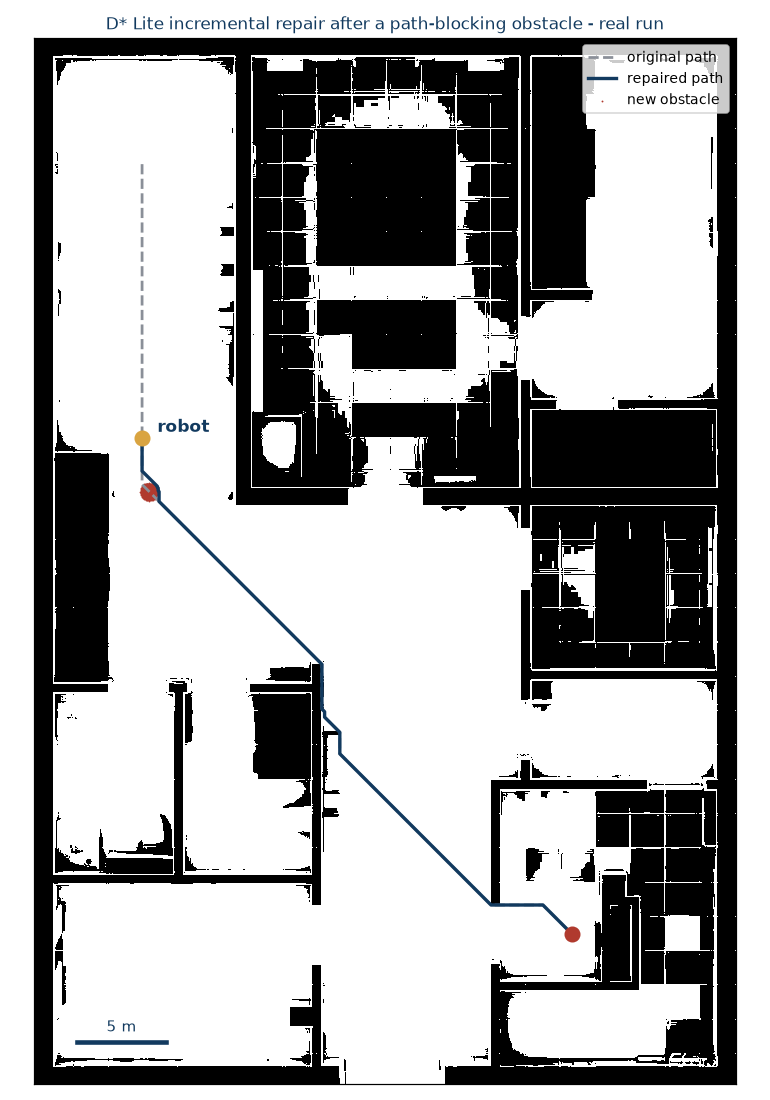
\includegraphics[width=0.58\linewidth]{replan_obstacle.png}
\caption{\small A real run on the repository's map. The dashed line was the original route. Something appears in the way (red), and the repaired route (solid) goes around it. This recovery cost 256 examined positions, because everything the planner already knew about the rest of the building was still true and was reused.}
\end{figure}

That is the entire idea, and stated like that it sounds like it should simply win. The interesting work is finding out whether it actually does, and by how much, and where it does not.

\section{Measuring it without fooling yourself}

It is easy to build a comparison that flatters the answer you want. This one is set up to make that hard:

\begin{itemize}[leftmargin=1.4em,itemsep=2pt]
\item \textbf{200 journeys}, with randomly chosen but reproducible start and end points at least 15 metres apart. The randomness is seeded, so anyone running it gets the identical set of journeys.
\item \textbf{Eight interruptions per journey}. The robot advances along its route, then an obstacle appears further ahead \emph{on the path it is currently following}, so the interruption always genuinely matters. There is no padding the numbers with changes the robot could have ignored.
\item \textbf{Both planners face the identical situation}, replanning from the same position on a byte-for-byte identical map.
\item \textbf{The order is alternated} on every event, because whichever algorithm runs second benefits from a warmed-up processor. Alternating cancels that out.
\item \textbf{Every event checks that both routes are equally good.} If the two ever disagree on the quality of the best available path, the benchmark fails and reports an error.
\end{itemize}

That last point deserves emphasis. It would be easy to look fast by cutting corners and producing slightly worse routes. Here, the two planners' answers were compared on all 1,716 measurements and matched every time. The comparison is between two planners that both find the genuinely best route, one of them faster.

\section{How much faster}

Across 1,493 interruptions:

\begin{center}
\small
\begin{tabular}{lrrr}
\toprule
& first route & typical recovery & positions examined \\
\midrule
Replan from scratch & 12.2 ms & 2.72 ms & 41,298 \\
Repair (D* Lite) & 33.3 ms & \textbf{0.245 ms} & \textbf{3,679} \\
\bottomrule
\end{tabular}
\end{center}

The typical recovery got about \textbf{eleven times faster}. Averaged across all interruptions, including the awkward ones, it is 4.3 times faster.

The averages and the typical case differ so much for a reason worth understanding. Replanning from scratch is wildly unpredictable: sometimes the new route is found almost immediately, sometimes it requires exploring half the building. Repair is consistent, because the work it does depends on the size of the change rather than the size of the building. For a robot, that consistency is worth as much as the speed. Unpredictable planning time is what produces a machine that lurches, stalls in doorways, and hesitates in front of people.

\section{The part most benchmarks leave out}

Repair does not always win. Out of 1,493 interruptions, it was faster on 993 of them.

That means it was slower on the other 500, and the reason is honest and structural. Repairing requires bookkeeping: noting what changed, working out which previous conclusions are now suspect, and revisiting them. When the change is trivial, and re-searching a short stretch of corridor would have been almost free anyway, that bookkeeping costs more than it saves.

There is a second cost, visible in the table above. The very first route, before anything has gone wrong, takes about 2.7 times longer to compute, because repair-based planning has to build a structure it can later repair.

\begin{figure}[t]
\centering
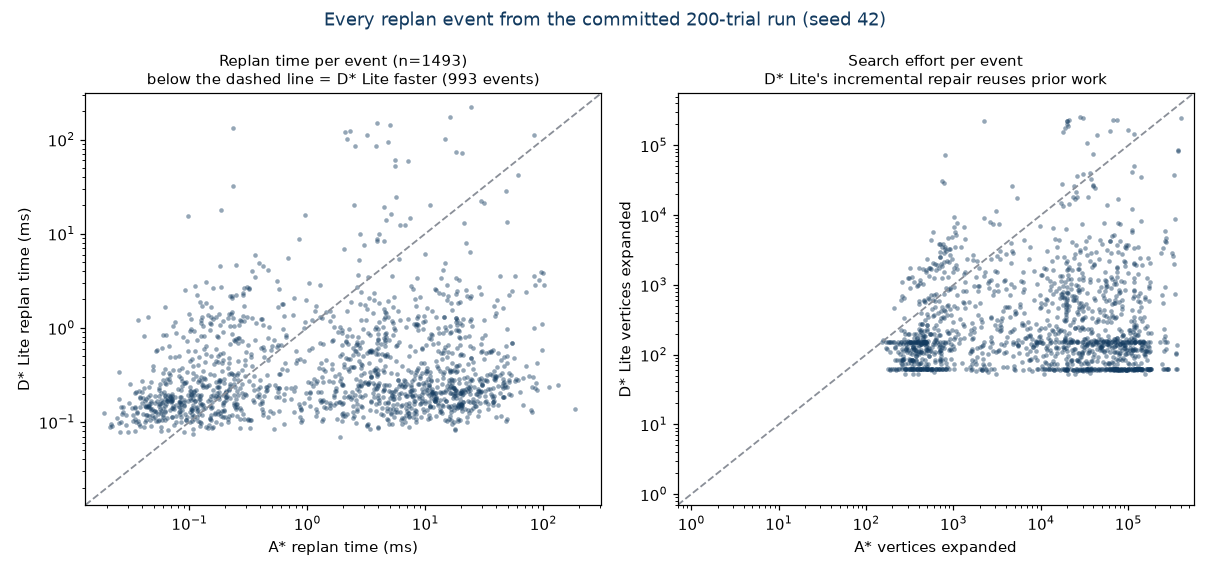
\includegraphics[width=\linewidth]{replan_scatter.png}
\caption{\small Every single interruption from the run, plotted individually. Each dot is one event. Below the dashed line, repair was faster; above it, replanning from scratch won. The right-hand panel shows why: repair's effort stays in a narrow band no matter how expensive the from-scratch search becomes, but that band has a floor, and cheap searches slip underneath it.}
\end{figure}

So the honest summary is not ``this algorithm is better''. It is: it costs more up front, it loses on the easy cases, and it wins overwhelmingly on the expensive ones, which happen to be exactly the cases that make a real robot stutter. Whether that trade is worth making depends on the robot, and the numbers to decide it are all published.

\section{The bug that was hiding inside a square root}

One more thing turned up in this project, and it is the sort of thing that is invisible until it is not.

Distances on a grid involve diagonals, and the length of a diagonal step is the square root of two: 1.41421356 and onwards forever. A computer cannot store that exactly. It stores something extremely close.

The repair algorithm constantly compares the priorities of competing positions, and those priorities frequently tie. When two values are mathematically identical but stored as almost-identical approximations, comparisons that should say ``equal'' say ``very slightly greater''. The consequence is not a crash or an obviously wrong answer. It is that a small piece of stale reasoning stays frozen in place, and the planner occasionally returns a route that is not quite the best one, for reasons nothing in the output explains.

The fix was to stop using fractions. Distances are measured in whole numbers, a straight step counted as 70 and a diagonal as 99, chosen so their ratio is close enough to the true one. Whole numbers compare exactly. The ties resolve correctly because they are genuinely equal.

\begin{quotebox}
Finding this needed a test that could not be argued with: 23,748 randomly generated scenarios producing 185,237 repairs, each one compared against a slow, simple, obviously correct reference method, demanding exact equality. Zero mismatches. The test runs automatically on every change to the code, and it is what caught the problem in the first place.
\end{quotebox}

\section{What this does not show}

Everything here is measured in simulation, on one building map, on one computer. The timings depend on the hardware; the counts of positions examined do not. No physical robot was involved.

The comparison also covers one specific situation, an obstacle appearing on the current route, because that is the situation repair-based planning exists for. Other kinds of change, such as an entire area becoming unavailable, are not measured here.

\section{Why it matters}

Robots that share space with people are interrupted constantly. Someone crosses a corridor, a door closes, a trolley is left where it should not be. Every one of those is a small demand to think again, and how gracefully a machine handles them determines whether people find it predictable or unnerving.

The claim in this project is modest and measured: for the interruptions that are expensive to recover from, repairing beats rebuilding by a wide margin, at a price paid up front and on the easy cases. Both halves of that sentence are in the published data, because a comparison that only reports the half that flatters it is not a measurement.

\vspace{6pt}
{\color{rule}\hrule height 1pt}
\vspace{6pt}

{\small Every trial, every timing, every figure, and the code that produces them are public, and reproduce exactly from the same random seed. This guide is part of a wider line of work on machines that behave predictably: a benchmark measuring \emph{how} language model planners fail, a safety layer that detects unsafe routes and recovers or halts, and this planning core, which supplies the provably correct alternatives that layer relies on.\\
Repository: \href{https://github.com/munawarkazmi/ros2-dynamic-path-planning}{github.com/munawarkazmi/ros2-dynamic-path-planning}}

\end{document}
